\documentclass[12pt]{article}

% Packages
\usepackage[margin=1in]{geometry}
\usepackage{amsmath, amsthm, amssymb, physics}
\usepackage{multirow, hhline, graphicx, listings}
\usepackage[table]{xcolor}

% Problem Box
\setlength{\fboxsep}{4pt}
\newsavebox{\mybox}
\newenvironment{problem}
    {\begin{lrbox}{\mybox}\begin{minipage}{0.98\textwidth}}
    {\end{minipage}\end{lrbox}\begin{center}\framebox[\textwidth]{\usebox{\mybox}}\end{center}}

% Options
\renewcommand{\thesubsection}{\thesection(\alph{subsection})}
\allowdisplaybreaks
\addtolength{\jot}{1em}
\theoremstyle{definition}

% Default Commands
\newtheorem{proposition}{Proposition}
\newtheorem{lemma}{Lemma}
\newcommand{\ds}{\displaystyle}
\newcommand{\isp}[1]{\quad\text{#1}\quad}
\newcommand{\N}{\mathbb{N}}
\newcommand{\Z}{\mathbb{Z}}
\newcommand{\Q}{\mathbb{Q}}
\newcommand{\R}{\mathbb{R}}
\newcommand{\C}{\mathbb{C}}
\newcommand{\eps}{\varepsilon}
\renewcommand{\phi}{\varphi}
\renewcommand{\emptyset}{\varnothing}

% Extra Commands



% Document Info
\title{Lab 3\\
    \large GEOG 191
}
\author{Harry Coleman}
\date{January 29, 2021}

% Begin Document
\begin{document}
\maketitle

\section{}
\begin{problem}
    Solve this problem using the simplex method, showing each steps of the algorithm. Use Xpress to verify your solution process
    \[\begin{array}{lrrcr}
        \textbf{Maximize}   & 3x_1  & +2x_2 \\
        \textbf{Subject to} & x_1   &       &\leq& 12 \\
                            & x_1   & +3x_2 &\leq& 45 \\
                            & 2x_1  & +x_2  &\leq& 30
    \end{array}\]
\end{problem}

We put this problem into standard form, introducing slack variables.
\[\begin{array}{*{11}{|c}|}
    \hline
    \text{Iteration} & \text{Row} & \text{BV} & Z & x_1 & x_2 & s_1 & s_2 & s_3 & \text{RHS} & \text{Ratio} \\\hline\hline
    \multirow{4}*{0}
    & 0 & Z   & 1 & -3 & -2 & 0 & 0 & 0 & 0  & \\\hhline{|~|*{10}{-}|}
    & 1 & s_1 & 0 & 1  & 0  & 1 & 0 & 0 & 12 & \\\hhline{|~|*{10}{-}|}
    & 2 & s_2 & 0 & 1  & 3  & 0 & 1 & 0 & 45 & \\\hhline{|~|*{10}{-}|}
    & 3 & s_3 & 0 & 2  & 1  & 0 & 0 & 1 & 30 & \\\hline
\end{array}\]

The entries for both $x_1$ and $x_2$ in the objective row are negative, but the entry for $x_1$ is larger, so it will be our incoming basic variable. The ratio test determines the outgoing basic variable, and we perform row operations to obtain the first iteration of the simplex method.
\[\begin{array}{*{11}{|c}|}
    \hline
    \text{Iteration} & \text{Row} & \text{BV} & Z & \cellcolor{gray!25} x_1 & x_2 & s_1 & s_2 & s_3 & \text{RHS} & \text{Ratio} \\\hline\hline
    \multirow{4}*{0}
    & 0 & Z   & 1 & -3 & -2 & 0 & 0 & 0 & 0  &    \\\hhline{|~|*{10}{-}|}
    & 1 & \cellcolor{gray!25}s_1 & 0 & 1  & 0  & 1 & 0 & 0 & 12 & 12 \\\hhline{|~|*{10}{-}|}
    & 2 & s_2 & 0 & 1  & 3  & 0 & 1 & 0 & 45 & 45 \\\hhline{|~|*{10}{-}|}
    & 3 & s_3 & 0 & 2  & 1  & 0 & 0 & 1 & 30 & 15 \\\hline
    \hline
    \multirow{4}*{1}
    & 0 & Z   & 1 & 0 & -2 & 3 & 0 & 0 & 36  & \\\hhline{|~|*{10}{-}|}
    & 1 & x_1 & 0 & 1  & 0  & 1 & 0 & 0 & 12 &  \\\hhline{|~|*{10}{-}|}
    & 2 & s_2 & 0 &  0 & 3  & -1 & 1 & 0 & 33 &  \\\hhline{|~|*{10}{-}|}
    & 3 & s_3 & 0 & 0  & 1  & -2 & 0 & 1 & 6 &  \\\hline
\end{array}\]

Our only possibility of improving the objective for the next iteration is taking $x_2$ as the incoming basic variable. Again, the ratio determines the outgoing basic variable, and and we perform row operations to obtain the second iteration.
\[\begin{array}{*{11}{|c}|}
    \hline
    \text{Iteration} & \text{Row} & \text{BV} & Z & x_1 & \cellcolor{gray!25}x_2 & s_1 & s_2 & s_3 & \text{RHS} & \text{Ratio} \\\hline\hline
    \multirow{4}*{1}
    & 0 & Z   & 1 & 0  & -2 & 3  & 0 & 0 & 36 &  \\\hhline{|~|*{10}{-}|}
    & 1 & x_1 & 0 & 1  & 0  & 1  & 0 & 0 & 12 &  - \\\hhline{|~|*{10}{-}|}
    & 2 & s_2 & 0 &  0 & 3  & -1 & 1 & 0 & 33 & 11 \\\hhline{|~|*{10}{-}|}
    & 3 & \cellcolor{gray!25}s_3 & 0 & 0  & 1  & -2 & 0 & 1 & 6  & 6 \\\hline
    \hline
    \multirow{4}*{2}
    & 0 & Z   & 1 & 0  & 0 & -1  & 0 & 2 & 48 & \\\hhline{|~|*{10}{-}|}
    & 1 & x_1 & 0 & 1  & 0  & 1  & 0 & 0 & 12 & \\\hhline{|~|*{10}{-}|}
    & 2 & s_2 & 0 &  0 & 0  & 5 & 1 & -3 & 15 & \\\hhline{|~|*{10}{-}|}
    & 3 & x_2 & 0 & 0  & 1  & -2 & 0 & 1 & 6  & \\\hline
\end{array}\]

Continuing the process, $s_1$ is our next incoming basic variable.
\[\begin{array}{*{11}{|c}|}
    \hline
    \text{Iteration} & \text{Row} & \text{BV} & Z & x_1 & x_2 & \cellcolor{gray!25}s_1 & s_2 & s_3 & \text{RHS} & \text{Ratio} \\\hline\hline
    \multirow{4}*{2}
    & 0 & Z   & 1 & 0  & 0 & -1  & 0 & 2 & 48 & \\\hhline{|~|*{10}{-}|}
    & 1 & x_1 & 0 & 1  & 0  & 1  & 0 & 0 & 12 & 12 \\\hhline{|~|*{10}{-}|}
    & 2 & \cellcolor{gray!25}s_2 & 0 &  0 & 0  & 5 & 1 & -3 & 15 & 3 \\\hhline{|~|*{10}{-}|}
    & 3 & x_2 & 0 & 0  & 1  & -2 & 0 & 1 & 6  & - \\\hline
    \hline
    \multirow{4}*{3}
    & 0 & Z   & 1 & 0  & 0 & 0  & 0.2 & 1.4 & 51 & \\\hhline{|~|*{10}{-}|}
    & 1 & x_1 & 0 & 1  & 0  & 0  & -0.2 & 0.6 & 9 & \\\hhline{|~|*{10}{-}|}
    & 2 & s_1 & 0 &  0 & 0  & 1 & 0.2 & -0.6 & 3 & \\\hhline{|~|*{10}{-}|}
    & 3 & x_2 & 0 & 0  & 1  & 0 & 0.4 & -0.2 & 12  & \\\hline
\end{array}\]

The objective cannot be improved since no variables have negative entries in the objective row. Thus, an objective value of $Z = 51$ is optimal and attained by $x_1 = 9$, $x_2 = 12$. Additionally, we have the basic variable $s_1 = 3$ and the nonbasic variables $s_2 = s_3 = 0$. We verify this result with Xpress in the following two ways.

\newpage

First, we implement the linear program as presented in the problem, i.e., with inequality constraints and only the variables $x_1$ and $x_2$.\\

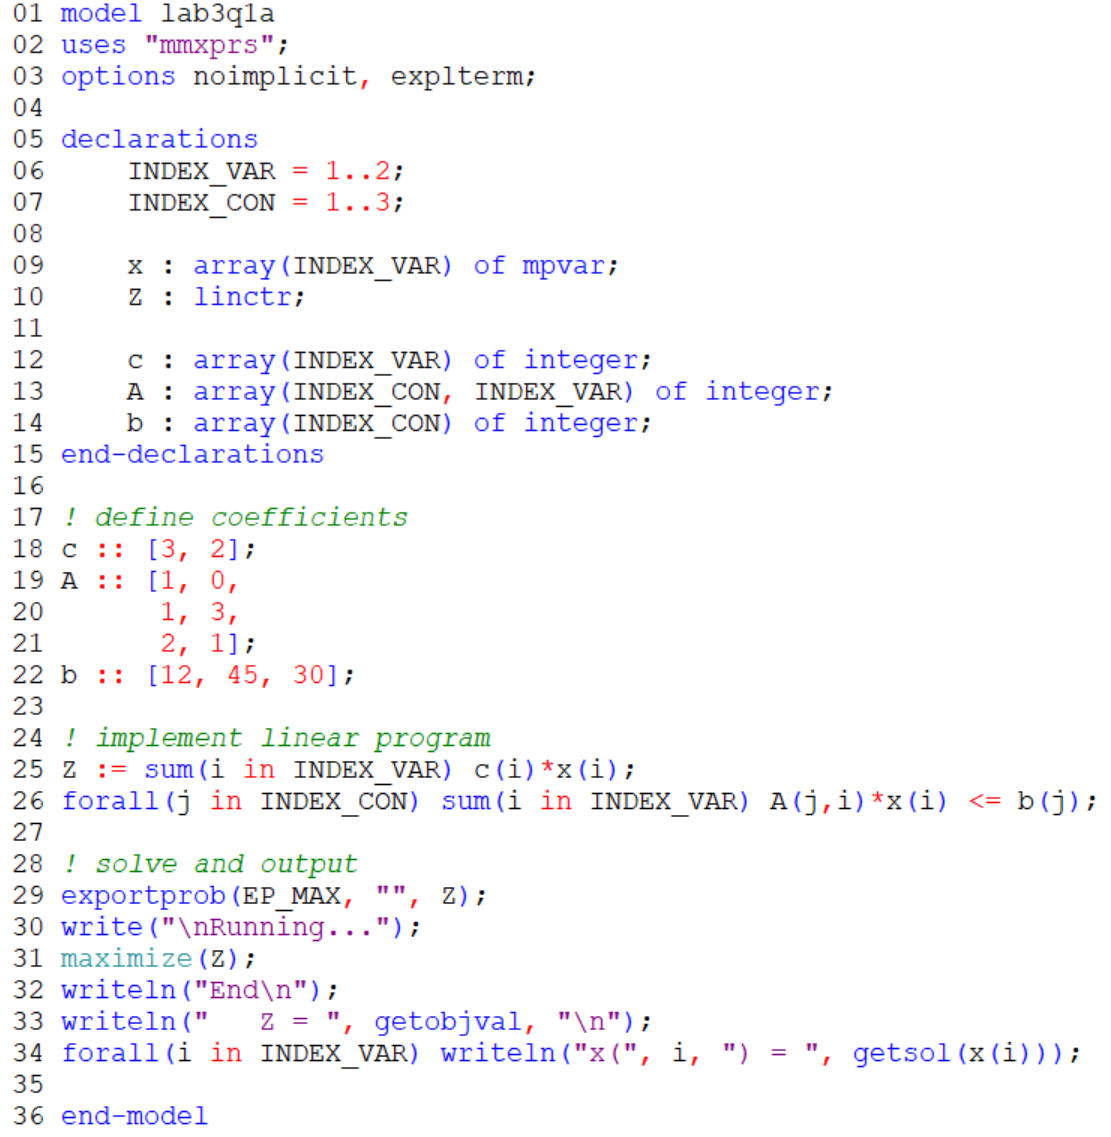
\includegraphics[scale=0.7]{code1a.png}\\
The output of this code is the following:

\lstset{basicstyle=\ttfamily}
\begin{lstlisting}
       Z = 51
    
    x(1) = 9
    x(2) = 12
\end{lstlisting}

\newpage

Second, we implement the linear program in standard augmented form, i.e., with equality constraints and added slack variables $s_1$, $s_2$, and $s_3$.\\

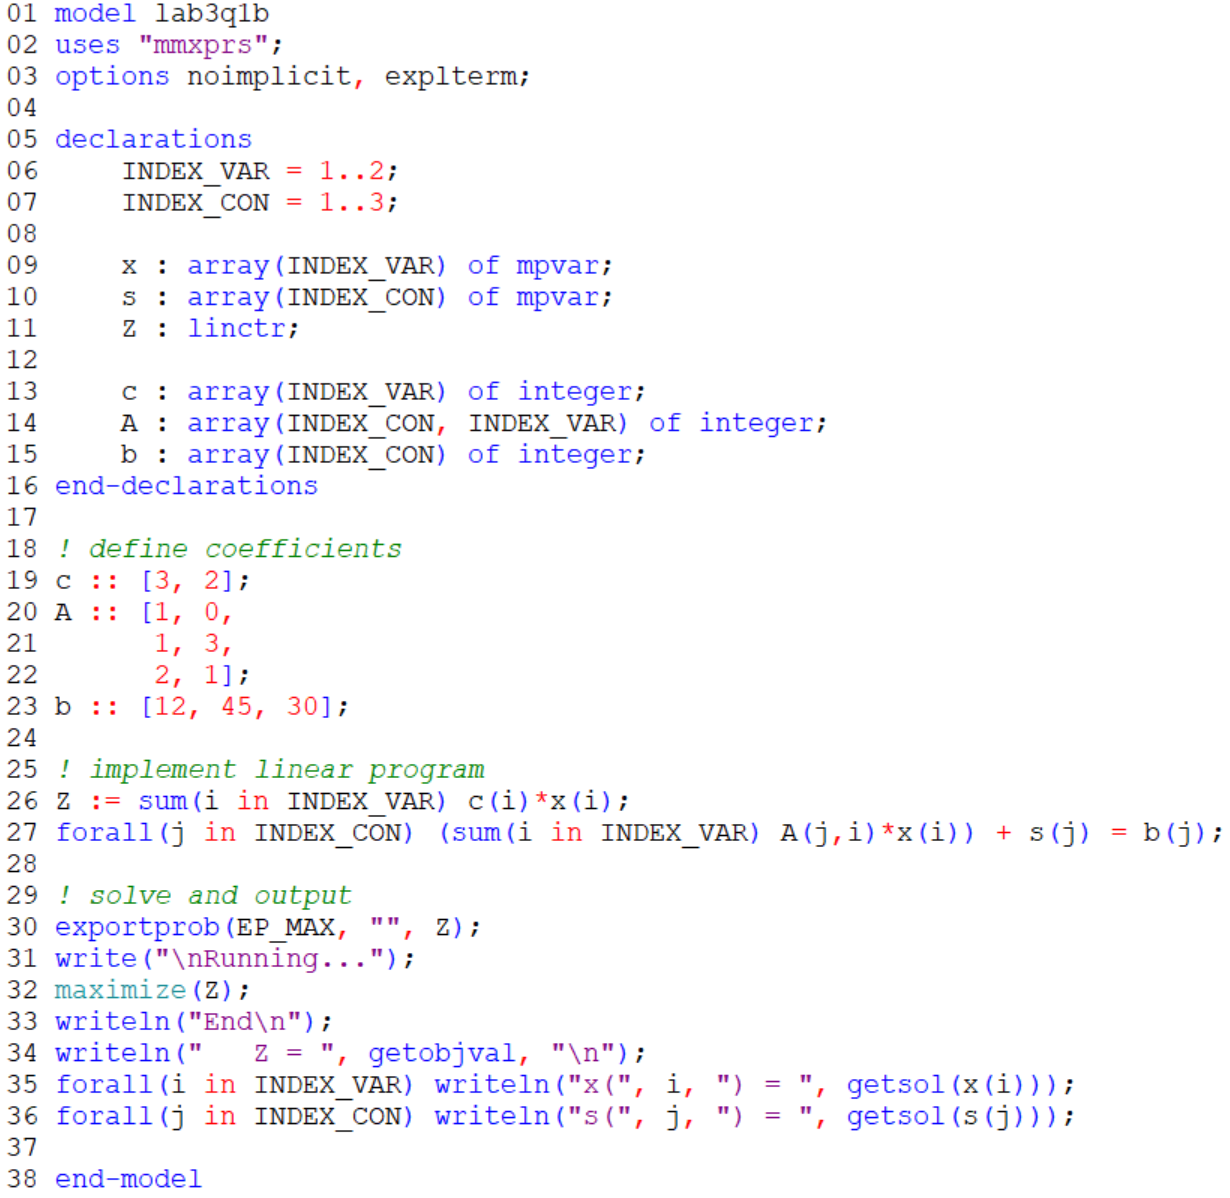
\includegraphics[scale=0.7]{code1b.png}\\
The output of this code is the following:

\lstset{basicstyle=\ttfamily}
\begin{lstlisting}
       Z = 51
    
    x(1) = 9
    x(2) = 12
    s(1) = 3
    s(2) = 0
    s(3) = 0
\end{lstlisting}


\newpage
\section{}
\begin{problem}
    Solve this problem using the simplex method, showing each steps of the algorithm. Use Xpress to verify your solution process
    \[\begin{array}{lrrrcr}
        \textbf{Maximize}   & 2x_1  & -2x_2 & +4x_3 \\
        \textbf{Subject to} & -x_1  & +x_2  & +x_3 &\leq& 20 \\
                            & 2x_1  & -x_2  & +x_3 &\leq& 10 \\
                            & x_1   & +x_2  & +x_3 &\leq& 60
    \end{array}\]
\end{problem}

We put this problem into standard form, introducing slack variables.
\[\begin{array}{*{12}{|c}|}
    \hline
    \text{Iteration} & \text{Row} & \text{BV} & Z & x_1 & x_2 & x_3 & s_1 & s_2 & s_3 & \text{RHS} & \text{Ratio} \\\hline\hline
    \multirow{4}*{0}
    & 0 & Z   & 1 & -2 & 2  & -4 & 0 & 0 & 0 & 0  & \\\hhline{|~|*{11}{-}|}
    & 1 & s_1 & 0 & -1 & 1  & 1  & 1 & 0 & 0 & 20 & \\\hhline{|~|*{11}{-}|}
    & 2 & s_2 & 0 & 2  & -1 & 1  & 0 & 1 & 0 & 10 & \\\hhline{|~|*{11}{-}|}
    & 3 & s_3 & 0 & 1  & 1  & 1  & 0 & 0 & 1 & 60 & \\\hline
\end{array}\]

The variable with the largest negative entry in the objective row is $x_3$, so it will be our first entering basic variable.

\[\begin{array}{*{12}{|c}|}
    \hline
    \text{Iteration} & \text{Row} & \text{BV} & Z & x_1 & x_2 & \cellcolor{gray!25}x_3 & s_1 & s_2 & s_3 & \text{RHS} & \text{Ratio} \\\hline\hline
    \multirow{4}*{0}
    & 0 & Z   & 1 & -2 & 2  & -4 & 0 & 0 & 0 & 0  & \\\hhline{|~|*{11}{-}|}
    & 1 & s_1 & 0 & -1 & 1  & 1  & 1 & 0 & 0 & 20 & 20 \\\hhline{|~|*{11}{-}|}
    & 2 & \cellcolor{gray!25}s_2 & 0 & 2  & -1 & 1  & 0 & 1 & 0 & 10 & 10 \\\hhline{|~|*{11}{-}|}
    & 3 & s_3 & 0 & 1  & 1  & 1  & 0 & 0 & 1 & 60 & 60 \\\hline
    \hline
    \multirow{4}*{1}
    & 0 & Z   & 1 & 8 & -2  & 0 & 0 & 4 & 0 & 40 & \\\hhline{|~|*{11}{-}|}
    & 1 & s_1 & 0 & -3 & 2  & 0  & 1 & -1 & 0 & 10 & \\\hhline{|~|*{11}{-}|}
    & 2 & x_3 & 0 & 2  & -1 & 1  & 0 & 1 & 0 & 10 & \\\hhline{|~|*{11}{-}|}
    & 3 & s_3 & 0 & -1  & 2  & 0  & 0 & -1 & 1 & 50 & \\\hline
\end{array}\]

The only option for the next basic variable is $x_2$.
\[\begin{array}{*{12}{|c}|}
    \hline
    \text{Iteration} & \text{Row} & \text{BV} & Z & x_1 & \cellcolor{gray!25}x_2 & x_3 & s_1 & s_2 & s_3 & \text{RHS} & \text{Ratio} \\\hline\hline
    \multirow{4}*{1}
    & 0 & Z   & 1 & 8 & -2  & 0 & 0 & 4 & 0 & 40 & \\\hhline{|~|*{11}{-}|}
    & 1 & \cellcolor{gray!25}s_1 & 0 & -3 & 2  & 0  & 1 & -1 & 0 & 10 & 5 \\\hhline{|~|*{11}{-}|}
    & 2 & x_3 & 0 & 2  & -1 & 1  & 0 & 1 & 0 & 10 & - \\\hhline{|~|*{11}{-}|}
    & 3 & s_3 & 0 & -1  & 2  & 0  & 0 & -1 & 1 & 50 & 25 \\\hline
    \hline
    \multirow{4}*{2}
    & 0 & Z   & 1 & 5 & 0  & 0 & 1 & 3 & 0 & 50 & \\\hhline{|~|*{11}{-}|}
    & 1 & x_2 & 0 & -1.5 & 1  & 0  & 0.5 & -0.5 & 0 & 5 & \\\hhline{|~|*{11}{-}|}
    & 2 & x_3 & 0 & 0.5  & 0 & 1  & 0.5 & 0.5 & 0 & 15 & \\\hhline{|~|*{11}{-}|}
    & 3 & s_3 & 0 & 2  & 0  & 0  & -1 & 0 & 1 & 40 & \\\hline
\end{array}\]

There are no more negative entries for variables in the objective row. Thus, an objective value of $Z = 50$ is optimal and is attained by $x_1 = 0$, $x_2 = 5$, $x_3 = 15$. Additionally, we have the basic variable $s_3 = 40$ and nonbasic variables $s_1 = s_2 = 0$. We verify this results with Xpress.

\newpage

As before, we first give an implementation with inequality constraints and only the variables $x_1$, $x_2$, and $x_3$.\\

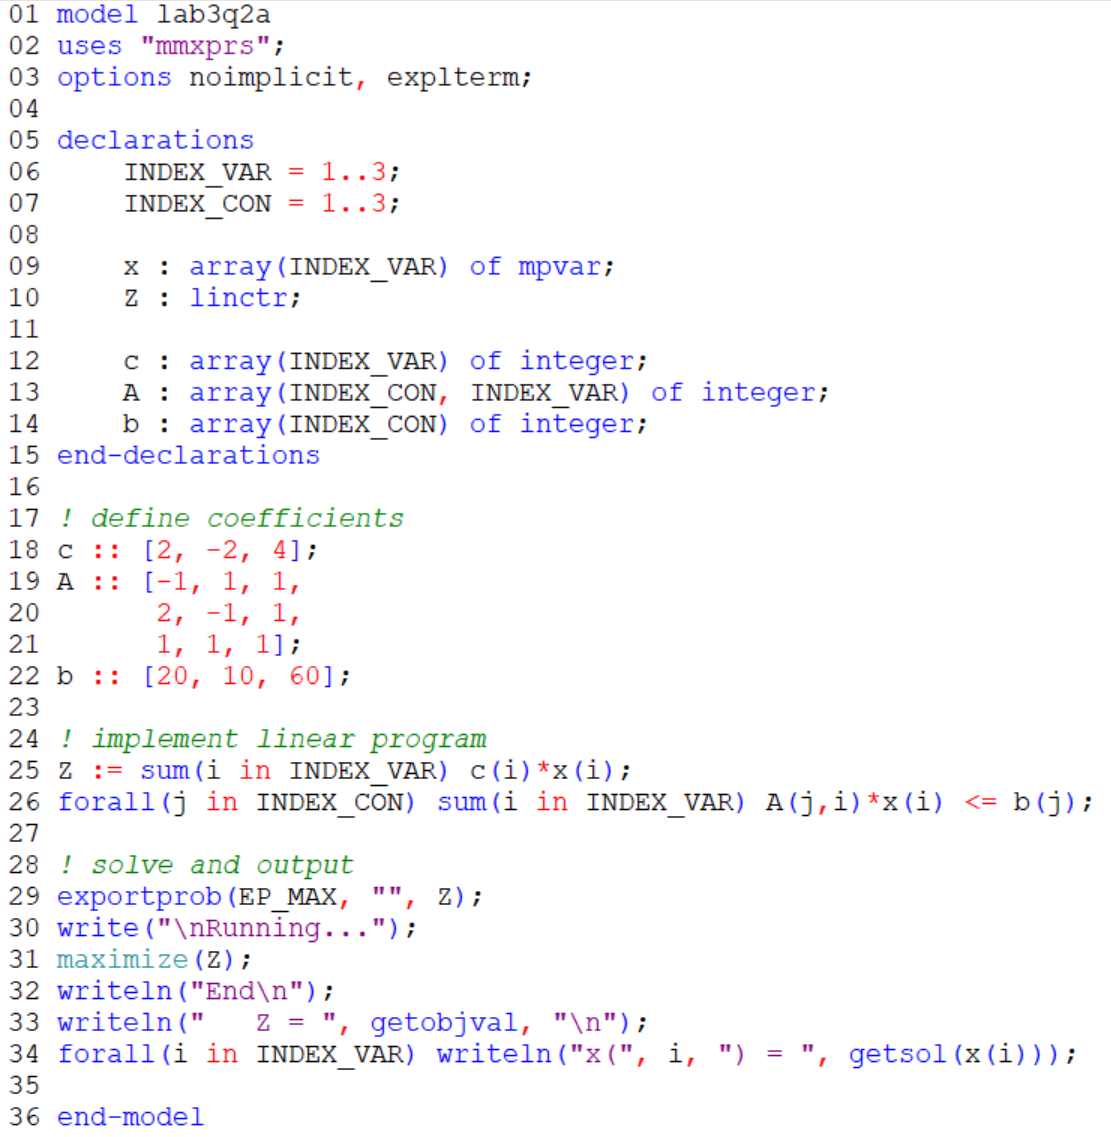
\includegraphics[scale=0.7]{code2a.png}\\
The output of this code is the following:

\lstset{basicstyle=\ttfamily}
\begin{lstlisting}
       Z = 50
    
    x(1) = 0
    x(2) = 5
    x(3) = 15
\end{lstlisting}

\newpage

Also as before, we now give an implementation with equality constraints and added slack variables $s_1$, $s_2$, and $s_3$.\\

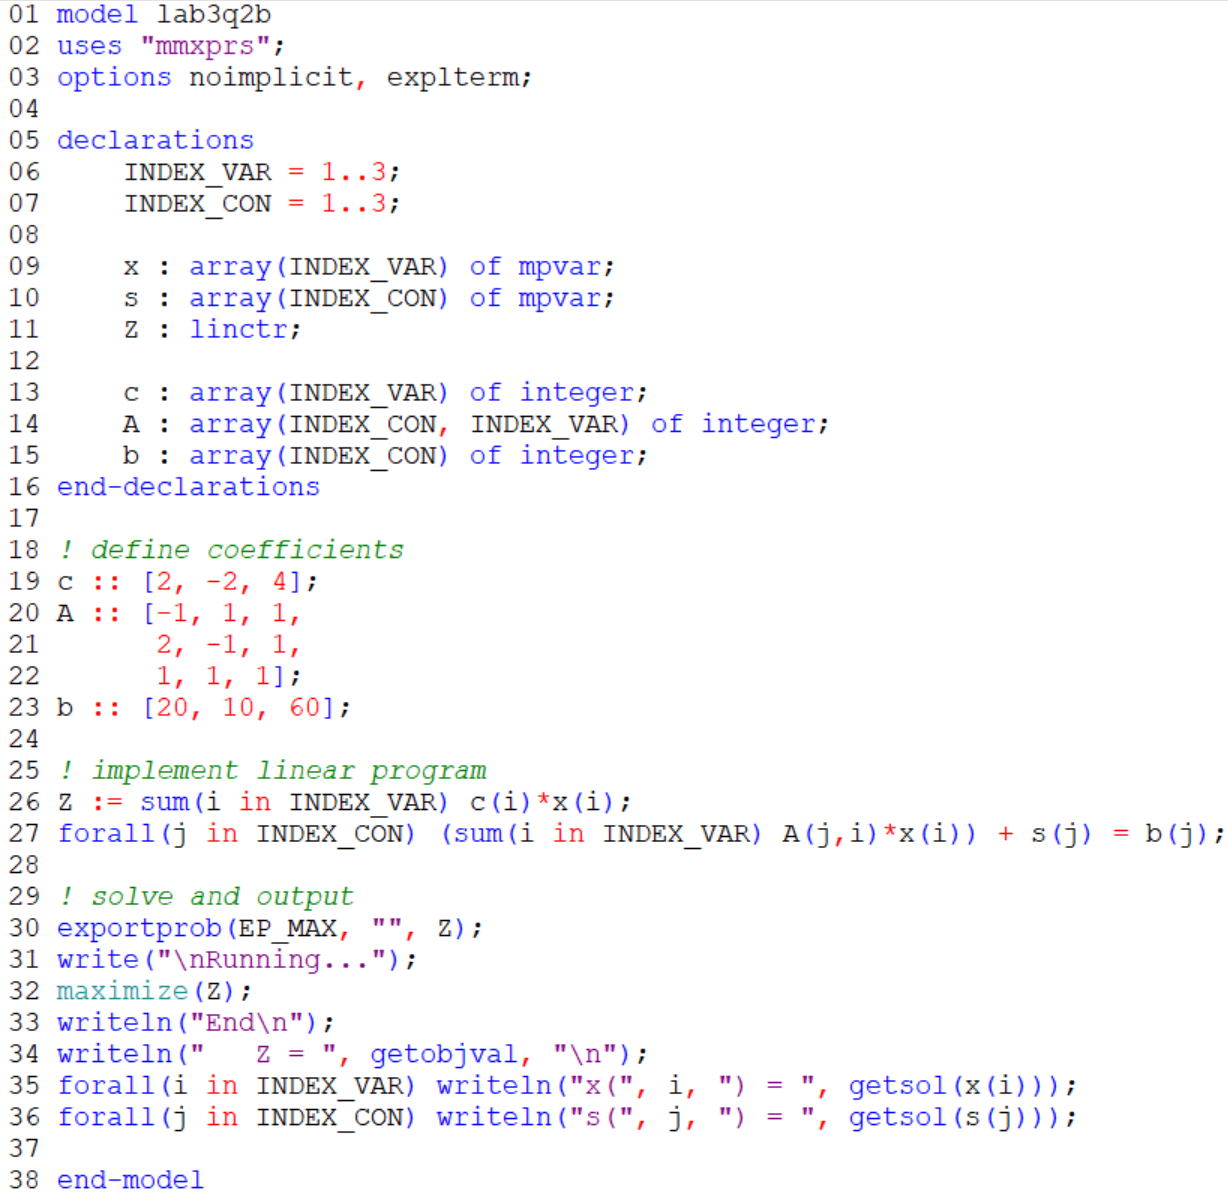
\includegraphics[scale=0.7]{code2b.png}\\
The output of this code is the following:
\begin{lstlisting}
       Z = 50
    
    x(1) = 0
    x(2) = 5
    x(3) = 15
    s(1) = 0
    s(2) = 0
    s(3) = 40
\end{lstlisting}

\end{document}